\documentclass{article}\usepackage{graphicx, color}
%% maxwidth is the original width if it is less than linewidth
%% otherwise use linewidth (to make sure the graphics do not exceed the margin)
\makeatletter
\def\maxwidth{ %
  \ifdim\Gin@nat@width>\linewidth
    \linewidth
  \else
    \Gin@nat@width
  \fi
}
\makeatother

\IfFileExists{upquote.sty}{\usepackage{upquote}}{}
\definecolor{fgcolor}{rgb}{0.2, 0.2, 0.2}
\newcommand{\hlnumber}[1]{\textcolor[rgb]{0,0,0}{#1}}%
\newcommand{\hlfunctioncall}[1]{\textcolor[rgb]{0.501960784313725,0,0.329411764705882}{\textbf{#1}}}%
\newcommand{\hlstring}[1]{\textcolor[rgb]{0.6,0.6,1}{#1}}%
\newcommand{\hlkeyword}[1]{\textcolor[rgb]{0,0,0}{\textbf{#1}}}%
\newcommand{\hlargument}[1]{\textcolor[rgb]{0.690196078431373,0.250980392156863,0.0196078431372549}{#1}}%
\newcommand{\hlcomment}[1]{\textcolor[rgb]{0.180392156862745,0.6,0.341176470588235}{#1}}%
\newcommand{\hlroxygencomment}[1]{\textcolor[rgb]{0.43921568627451,0.47843137254902,0.701960784313725}{#1}}%
\newcommand{\hlformalargs}[1]{\textcolor[rgb]{0.690196078431373,0.250980392156863,0.0196078431372549}{#1}}%
\newcommand{\hleqformalargs}[1]{\textcolor[rgb]{0.690196078431373,0.250980392156863,0.0196078431372549}{#1}}%
\newcommand{\hlassignement}[1]{\textcolor[rgb]{0,0,0}{\textbf{#1}}}%
\newcommand{\hlpackage}[1]{\textcolor[rgb]{0.588235294117647,0.709803921568627,0.145098039215686}{#1}}%
\newcommand{\hlslot}[1]{\textit{#1}}%
\newcommand{\hlsymbol}[1]{\textcolor[rgb]{0,0,0}{#1}}%
\newcommand{\hlprompt}[1]{\textcolor[rgb]{0.2,0.2,0.2}{#1}}%

\usepackage{framed}
\makeatletter
\newenvironment{kframe}{%
 \def\at@end@of@kframe{}%
 \ifinner\ifhmode%
  \def\at@end@of@kframe{\end{minipage}}%
  \begin{minipage}{\columnwidth}%
 \fi\fi%
 \def\FrameCommand##1{\hskip\@totalleftmargin \hskip-\fboxsep
 \colorbox{shadecolor}{##1}\hskip-\fboxsep
     % There is no \\@totalrightmargin, so:
     \hskip-\linewidth \hskip-\@totalleftmargin \hskip\columnwidth}%
 \MakeFramed {\advance\hsize-\width
   \@totalleftmargin\z@ \linewidth\hsize
   \@setminipage}}%
 {\par\unskip\endMakeFramed%
 \at@end@of@kframe}
\makeatother

\definecolor{shadecolor}{rgb}{.97, .97, .97}
\definecolor{messagecolor}{rgb}{0, 0, 0}
\definecolor{warningcolor}{rgb}{1, 0, 1}
\definecolor{errorcolor}{rgb}{1, 0, 0}
\newenvironment{knitrout}{}{} % an empty environment to be redefined in TeX

\usepackage{alltt}

\title{STATS 209 - Midterm}
\author{Rene Kizilcec}
\date{Feb 14, 2013}

\begin{document}
\maketitle 







\section*{QUESTION 1}
\subsection*{part a}
Let X1=fitness, X2=stress, X3=illness
\begin{knitrout}
\definecolor{shadecolor}{rgb}{0.969, 0.969, 0.969}\color{fgcolor}\begin{kframe}
\begin{alltt}
r12=-.13
r13=-.29
r23=.34
r13.2=(r13-r12*r23)/((1-r12^2)*(1-r23^2))^.5
r13.2
\end{alltt}
\begin{verbatim}
[1] -0.2636
\end{verbatim}
\end{kframe}
\end{knitrout}

-.264 is not much less than -.29

Obtain CI by converting r to Fisher z' and back.
\begin{knitrout}
\definecolor{shadecolor}{rgb}{0.969, 0.969, 0.969}\color{fgcolor}\begin{kframe}
\begin{alltt}
\hlfunctioncall{r.con}(-.264,373) 
\end{alltt}
\begin{verbatim}
[1] -0.3560 -0.1669
\end{verbatim}
\end{kframe}
\end{knitrout}

95\% CI does not include 0. No evidence for fitness-illness association to be spurious.

\subsection*{part b}
\begin{knitrout}
\definecolor{shadecolor}{rgb}{0.969, 0.969, 0.969}\color{fgcolor}\begin{kframe}
\begin{alltt}
corPred=\hlfunctioncall{matrix}(
    \hlfunctioncall{c}(1,-.03,.39,-.05,-.03,1,.07,-.23,.39,.07,1,-.13,-.05,-.23,-.13,1),
    byrow=F,ncol=4)
corPred
\end{alltt}
\begin{verbatim}
      [,1]  [,2]  [,3]  [,4]
[1,]  1.00 -0.03  0.39 -0.05
[2,] -0.03  1.00  0.07 -0.23
[3,]  0.39  0.07  1.00 -0.13
[4,] -0.05 -0.23 -0.13  1.00
\end{verbatim}
\begin{alltt}
corResp=\hlfunctioncall{matrix}(\hlfunctioncall{c}(-.08,-.16,-.29,.34),ncol=1,byrow=F)
coefs = \hlfunctioncall{t}(corResp)%*%\hlfunctioncall{solve}(corPred)
coefs 
\end{alltt}
\begin{verbatim}
        [,1]     [,2]    [,3]   [,4]
[1,] 0.03381 -0.07387 -0.2602 0.2909
\end{verbatim}
\begin{alltt}
\hlcomment{# same as direct effects in Table 5.2. (kleine p.121)}

\hlcomment{# compute R-squared (not adjusted)}
rsq=coefs%*%corResp
rsq
\end{alltt}
\begin{verbatim}
       [,1]
[1,] 0.1835
\end{verbatim}
\begin{alltt}
\hlcomment{# covariance matrix with standardized values}
covB = \hlfunctioncall{as.numeric}(1-rsq)*\hlfunctioncall{solve}(corPred)
covB
\end{alltt}
\begin{verbatim}
         [,1]     [,2]     [,3]    [,4]
[1,]  0.96694  0.05844 -0.37958 0.01244
[2,]  0.05844  0.86716 -0.05817 0.19481
[3,] -0.37958 -0.05817  0.98101 0.09517
[4,]  0.01244  0.19481  0.09517 0.87433
\end{verbatim}
\begin{alltt}
\hlcomment{# Note that standard errors for standardized coeffs }
\hlcomment{# are just square roots of the diagonals adjusted for sample size}

\hlcomment{# standardized SE for Excercise}
\hlfunctioncall{sqrt}((covB[1,1]/(373))*(373 / (373-4))) 
\end{alltt}
\begin{verbatim}
[1] 0.05119
\end{verbatim}
\begin{alltt}
\hlcomment{# standardized SE for Hardiness}
\hlfunctioncall{sqrt}((covB[2,2]/(373))*(373 / (373-4))) 
\end{alltt}
\begin{verbatim}
[1] 0.04848
\end{verbatim}
\begin{alltt}
\hlcomment{# standardized SE for Fitness}
\hlfunctioncall{sqrt}((covB[3,3]/(373))*(373 / (373-4))) 
\end{alltt}
\begin{verbatim}
[1] 0.05156
\end{verbatim}
\begin{alltt}
\hlcomment{# standardized SE for Stress}
\hlfunctioncall{sqrt}((covB[4,4]/(373))*(373 / (373-4))) 
\end{alltt}
\begin{verbatim}
[1] 0.04868
\end{verbatim}
\begin{alltt}

\hlcomment{# c-c' = beta32 * beta13.2 =a*b #where X1=ill,X2=fit,X3=stress}
\hlcomment{# using Tab 5.2.}
mediation=-.11*.29 \hlcomment{# = -0.0319}
\hlcomment{#need to obtain se of fitness, do regression on stress}
newCov=\hlfunctioncall{cbind}(\hlfunctioncall{rbind}(corPred,\hlfunctioncall{t}(corResp)),\hlfunctioncall{c}(corResp,1))
newPred=newCov[-4,-4]
newPred
\end{alltt}
\begin{verbatim}
      [,1]  [,2]  [,3]  [,4]
[1,]  1.00 -0.03  0.39 -0.08
[2,] -0.03  1.00  0.07 -0.16
[3,]  0.39  0.07  1.00 -0.29
[4,] -0.08 -0.16 -0.29  1.00
\end{verbatim}
\begin{alltt}
newResp=\hlfunctioncall{t}(\hlfunctioncall{t}(newCov[-4,4]))
newCoefs = \hlfunctioncall{t}(newResp)%*%\hlfunctioncall{solve}(newPred)
newRsq=newCoefs%*%newResp
newRsq
\end{alltt}
\begin{verbatim}
       [,1]
[1,] 0.1485
\end{verbatim}
\begin{alltt}
\hlcomment{# covariance matrix with standardized values}
newCov = \hlfunctioncall{as.numeric}(1-newRsq)*\hlfunctioncall{solve}(newPred)

\hlcomment{# standardized SE for Fitness}
\hlfunctioncall{sqrt}((newCov[3,3]/(373))*(373 / (373-4))) 
\end{alltt}
\begin{verbatim}
[1] 0.05443
\end{verbatim}
\begin{alltt}

\hlcomment{# var(c-c')=b^2 Sa^2 + a^2 Sb^2}
sobel=(-.11)^2 * 0.05442998 + .29^2 *.048677 
sobel \hlcomment{# standardized}
\end{alltt}
\begin{verbatim}
[1] 0.004752
\end{verbatim}
\end{kframe}
\end{knitrout}

There mediation effects seems to be rather weak.

\subsection*{part c}
I would expect measurement error to spuriously increase the mediation effect, or even reverse the direction.


\newpage
\section*{QUESTION 2}
\subsection*{part 1}
From the results in Table 3 (use 18-month change from baseline) and Table 5 (use 18-month systolic) estimate the dose-response relation for decrease in systolic blood pressure for each unit decrease in salt intake (as measured by sodium excretion).\\
-43.9 = difference between trt and ctr salt (18 months)\\
-2.06 = difference between trt and ctr blood pressure (18 months)\\
2.06/43.9 = 0.047 reduction in blood pressure for 1 unit reduction in salt intake\\

\emph{What strong assumption did you need to make to justify this estimator?}\\
I assumed a linear dose-response relation (as opposed to a different functional form).\\

\emph{Briefly justify that assumption for this study?}
\begin{knitrout}
\definecolor{shadecolor}{rgb}{0.969, 0.969, 0.969}\color{fgcolor}\begin{kframe}
\begin{alltt}
2.03/((154.6-103)-(156.4-159.3))    \hlcomment{# (6months)}
\end{alltt}
\begin{verbatim}
[1] 0.03725
\end{verbatim}
\begin{alltt}
1.9/((154.6-100.2)-(156.4-152.1))   \hlcomment{# (12months)}
\end{alltt}
\begin{verbatim}
[1] 0.03792
\end{verbatim}
\begin{alltt}
2.06/((154.6-99.4)-(156.4-146.5))   \hlcomment{# (18months)}
\end{alltt}
\begin{verbatim}
[1] 0.04547
\end{verbatim}
\end{kframe}
\end{knitrout}

The doese-response relation measured after 6 and 12 months are very similar, which points at a linear functional form.\\
However, after 18 months, the relation becomes stronger. Note (!) that there is a mistake in Table 3, the "18-Month change from baseline" value for Control, does not correspond to thte difference between Baseline and 18-Month.


\subsection*{part 2}
\begin{knitrout}
\definecolor{shadecolor}{rgb}{0.969, 0.969, 0.969}\color{fgcolor}\begin{kframe}
\begin{alltt}
\hlcomment{#install.packages("mediation")}
\hlfunctioncall{library}(mediation)
\hlfunctioncall{data}(framing)
\hlfunctioncall{table}(framing$treat) \hlcomment{# yes, corresponds}
\end{alltt}
\begin{verbatim}

  0   1 
197  68 
\end{verbatim}
\begin{alltt}
\hlfunctioncall{dim}(framing) \hlcomment{# and yes, also corresponds}
\end{alltt}
\begin{verbatim}
[1] 265  15
\end{verbatim}
\end{kframe}
\end{knitrout}

Let us look at plots of these variables to see what might be going on. It looks like emotional stability is higher for those in the treatment condition (0=ctr, 1=trt) and even more so for those who decide to send a message (0=NotSend, 1=Send).
\begin{knitrout}
\definecolor{shadecolor}{rgb}{0.969, 0.969, 0.969}\color{fgcolor}\begin{kframe}
\begin{alltt}
\hlfunctioncall{par}(mfrow=\hlfunctioncall{c}(1,2))
\hlfunctioncall{boxplot}(framing$emo~framing$treat, main=\hlstring{"Emo for control/treatment"})
\hlfunctioncall{boxplot}(framing$emo~framing$cong_mesg, main=\hlstring{"Emo for NotSend/Send"})
\end{alltt}
\end{kframe}

{\centering 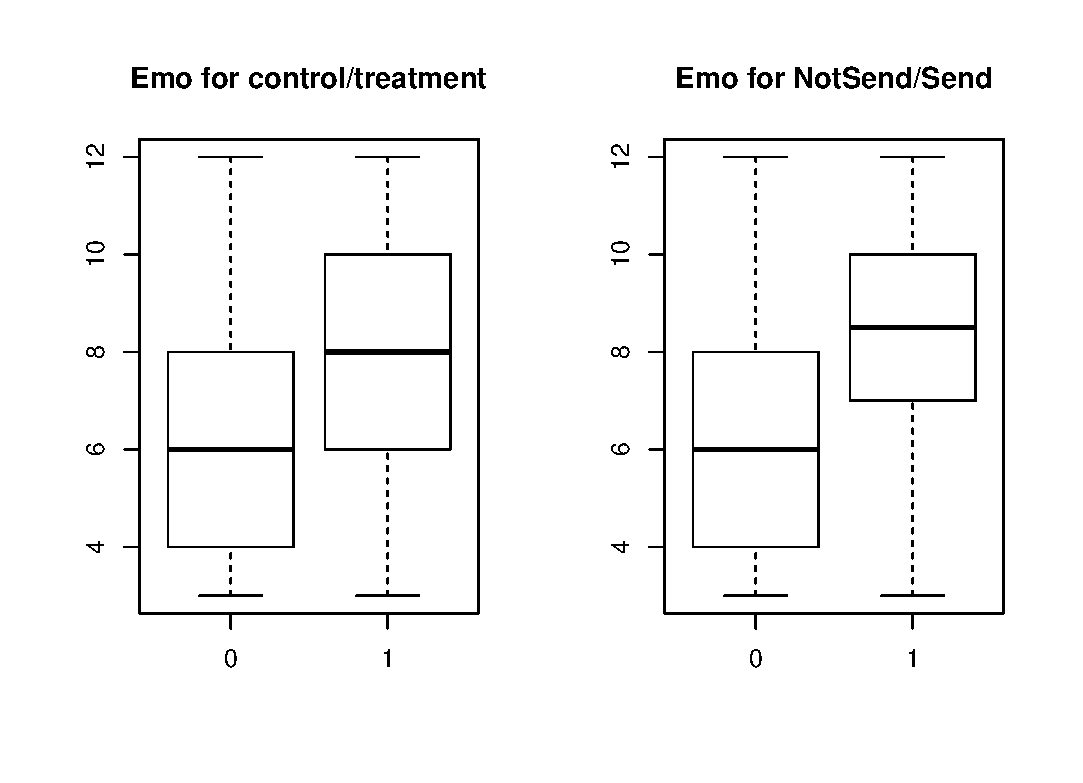
\includegraphics[width=\linewidth]{plots/unnamed-chunk-7} 

}



\end{knitrout}

\emph{Is there a significant effect of treatment on emo?}
\begin{knitrout}
\definecolor{shadecolor}{rgb}{0.969, 0.969, 0.969}\color{fgcolor}\begin{kframe}
\begin{alltt}
\hlfunctioncall{summary}(\hlfunctioncall{lm}(emo ~ treat,framing))
\end{alltt}
\begin{verbatim}

Call:
lm(formula = emo ~ treat, data = framing)

Residuals:
   Min     1Q Median     3Q    Max 
-5.074 -2.074 -0.074  1.926  5.406 

Coefficients:
            Estimate Std. Error t value Pr(>|t|)    
(Intercept)    6.594      0.193   34.23  < 2e-16 ***
treat          1.480      0.380    3.89  0.00013 ***
---
Signif. codes:  0 '***' 0.001 '**' 0.01 '*' 0.05 '.' 0.1 ' ' 1 

Residual standard error: 2.7 on 263 degrees of freedom
Multiple R-squared: 0.0544,	Adjusted R-squared: 0.0508 
F-statistic: 15.1 on 1 and 263 DF,  p-value: 0.000126 
\end{verbatim}
\end{kframe}
\end{knitrout}

Treatment effect significantly reduces anxiety (increases emo) $est=1.48, se=0.38, t=3.89$

\emph{Is there a significant effect of treatment on cong\_mesg?}
\begin{knitrout}
\definecolor{shadecolor}{rgb}{0.969, 0.969, 0.969}\color{fgcolor}\begin{kframe}
\begin{alltt}
\hlfunctioncall{summary}(\hlfunctioncall{lm}(cong_mesg ~ treat,framing)) 
\end{alltt}
\begin{verbatim}

Call:
lm(formula = cong_mesg ~ treat, data = framing)

Residuals:
   Min     1Q Median     3Q    Max 
-0.412 -0.305 -0.305  0.588  0.695 

Coefficients:
            Estimate Std. Error t value Pr(>|t|)    
(Intercept)   0.3046     0.0335    9.09   <2e-16 ***
treat         0.1072     0.0662    1.62     0.11    
---
Signif. codes:  0 '***' 0.001 '**' 0.01 '*' 0.05 '.' 0.1 ' ' 1 

Residual standard error: 0.47 on 263 degrees of freedom
Multiple R-squared: 0.00988,	Adjusted R-squared: 0.00612 
F-statistic: 2.63 on 1 and 263 DF,  p-value: 0.106 
\end{verbatim}
\end{kframe}
\end{knitrout}

No, treatment has no significant effect on cong\_mesg, $t=1.62, p=.11$

\emph{Estimate the effect on probability of sending congressional message of a unit change in "emo" (negative feelings).}
\begin{knitrout}
\definecolor{shadecolor}{rgb}{0.969, 0.969, 0.969}\color{fgcolor}\begin{kframe}
\begin{alltt}
\hlfunctioncall{summary}(\hlfunctioncall{lm}(cong_mesg ~ emo,framing)) 
\end{alltt}
\begin{verbatim}

Call:
lm(formula = cong_mesg ~ emo, data = framing)

Residuals:
   Min     1Q Median     3Q    Max 
-0.649 -0.334 -0.144  0.477  0.919 

Coefficients:
            Estimate Std. Error t value Pr(>|t|)    
(Intercept) -0.10814    0.07305   -1.48     0.14    
emo          0.06313    0.00974    6.48  4.4e-10 ***
---
Signif. codes:  0 '***' 0.001 '**' 0.01 '*' 0.05 '.' 0.1 ' ' 1 

Residual standard error: 0.439 on 263 degrees of freedom
Multiple R-squared: 0.138,	Adjusted R-squared: 0.135 
F-statistic:   42 on 1 and 263 DF,  p-value: 4.4e-10 
\end{verbatim}
\end{kframe}
\end{knitrout}

The prob. of sending message increases by 6.3\% points for each additional unit of emo. Note that at emo=0, the intercept (baseline prob.) is out of bound (below unit interval). This is a result of using OLS instead of logistic regression.\\

\emph{Compare the "path analysis" estimator (see week 3) for the encouragement design with the estimator you used in part 1.}\\
The estimator in part 1 is result of computing two difference-in-difference points and calculating the slope of straight line that passes though both points.
The 'path analysis' estimator is based on two regressions $BP \sim Salt + Group$, and $Salt\sim Group$.\\
However, these regressions reveal that the 'path analysis' coefficients are biased. There is support for a zero relation between treat and cong\_mesg here (like $\tau=0$ in class). Still, even under this assumption, the 'p.a.' estimator is biased, due to individual differences in cong\_mesg.\\

\emph{Why do the needed assumptions in this study seem far less reasonable than for the salt example?}
It seems unlikely that assignment to group (treat) has no effect on cong\_mesg because people are exposed to media stories in both conditions, which likely raises their awareness of current issues either way (ctr and trt) and thereby increase prob. of sending message. (however, this is not supported by the regression above)\\
An important individual difference that in this study is gender, given that changes in "emo" are likely to different between gender. (Females more emotional than males?) 
\begin{knitrout}
\definecolor{shadecolor}{rgb}{0.969, 0.969, 0.969}\color{fgcolor}\begin{kframe}
\begin{alltt}
\hlfunctioncall{boxplot}(framing$emo~framing$gender)
\end{alltt}
\end{kframe}

{\centering \includegraphics[width=\linewidth]{plots/unnamed-chunk-11} 

}



\end{knitrout}

It doesn't look like there is a gernder difference in emotional stability from this plot.\\

\emph{Repeat these questions just for the females in the study. Find anything different?}
\begin{knitrout}
\definecolor{shadecolor}{rgb}{0.969, 0.969, 0.969}\color{fgcolor}\begin{kframe}
\begin{alltt}
\hlfunctioncall{summary}(\hlfunctioncall{lm}(emo ~ treat,\hlfunctioncall{subset}(framing,gender==\hlstring{"female"}))) 
\end{alltt}
\begin{verbatim}

Call:
lm(formula = emo ~ treat, data = subset(framing, gender == "female"))

Residuals:
   Min     1Q Median     3Q    Max 
-4.921 -1.762  0.079  2.079  5.238 

Coefficients:
            Estimate Std. Error t value Pr(>|t|)    
(Intercept)    6.762      0.270   25.02   <2e-16 ***
treat          1.159      0.517    2.24    0.027 *  
---
Signif. codes:  0 '***' 0.001 '**' 0.01 '*' 0.05 '.' 0.1 ' ' 1 

Residual standard error: 2.72 on 137 degrees of freedom
Multiple R-squared: 0.0354,	Adjusted R-squared: 0.0283 
F-statistic: 5.02 on 1 and 137 DF,  p-value: 0.0266 
\end{verbatim}
\end{kframe}
\end{knitrout}

Significant and similar to above, 1.16 increase in emo (anxiety reduction) due to treatment.
\begin{knitrout}
\definecolor{shadecolor}{rgb}{0.969, 0.969, 0.969}\color{fgcolor}\begin{kframe}
\begin{alltt}
\hlfunctioncall{summary}(\hlfunctioncall{lm}(cong_mesg ~ treat,\hlfunctioncall{subset}(framing,gender==\hlstring{"female"}))) 
\end{alltt}
\begin{verbatim}

Call:
lm(formula = cong_mesg ~ treat, data = subset(framing, gender == 
    "female"))

Residuals:
   Min     1Q Median     3Q    Max 
-0.289 -0.277 -0.277  0.711  0.723 

Coefficients:
            Estimate Std. Error t value Pr(>|t|)    
(Intercept)   0.2772     0.0450    6.16  7.7e-09 ***
treat         0.0122     0.0861    0.14     0.89    
---
Signif. codes:  0 '***' 0.001 '**' 0.01 '*' 0.05 '.' 0.1 ' ' 1 

Residual standard error: 0.453 on 137 degrees of freedom
Multiple R-squared: 0.000148,	Adjusted R-squared: -0.00715 
F-statistic: 0.0202 on 1 and 137 DF,  p-value: 0.887 
\end{verbatim}
\end{kframe}
\end{knitrout}

Not significant (t=0.14), just like above.
\begin{knitrout}
\definecolor{shadecolor}{rgb}{0.969, 0.969, 0.969}\color{fgcolor}\begin{kframe}
\begin{alltt}
\hlfunctioncall{summary}(\hlfunctioncall{lm}(cong_mesg ~ emo,\hlfunctioncall{subset}(framing,gender==\hlstring{"female"})))
\end{alltt}
\begin{verbatim}

Call:
lm(formula = cong_mesg ~ emo, data = subset(framing, gender == 
    "female"))

Residuals:
   Min     1Q Median     3Q    Max 
-0.557 -0.276 -0.164  0.443  0.949 

Coefficients:
            Estimate Std. Error t value Pr(>|t|)    
(Intercept)  -0.1173     0.0997   -1.18     0.24    
emo           0.0562     0.0131    4.28  3.5e-05 ***
---
Signif. codes:  0 '***' 0.001 '**' 0.01 '*' 0.05 '.' 0.1 ' ' 1 

Residual standard error: 0.425 on 137 degrees of freedom
Multiple R-squared: 0.118,	Adjusted R-squared: 0.112 
F-statistic: 18.3 on 1 and 137 DF,  p-value: 3.47e-05 
\end{verbatim}
\end{kframe}
\end{knitrout}

Significant 5.6\% points prob. increase associated with additional unit emo. Similar to above. Not much different compared to above.

\newpage
\section*{QUESTION 3}
\begin{knitrout}
\definecolor{shadecolor}{rgb}{0.969, 0.969, 0.969}\color{fgcolor}\begin{kframe}
\begin{alltt}
\hlcomment{#install.packages("mlmRev")}
\hlfunctioncall{library}(mlmRev)
\hlfunctioncall{data}(Exam)
\end{alltt}
\end{kframe}
\end{knitrout}

Check if 'schavg' is really the school mean of 'standLRT'. Looks like schavg and mean(standLRT) correspond very well.
\begin{knitrout}
\definecolor{shadecolor}{rgb}{0.969, 0.969, 0.969}\color{fgcolor}\begin{kframe}
\begin{alltt}
\hlfunctioncall{ddply}(Exam, \hlfunctioncall{.}(school,schavg), summarize, \hlstring{"\hlfunctioncall{mean}(standLRT)"}=\hlfunctioncall{mean}(standLRT))
\end{alltt}
\begin{verbatim}
   school    schavg mean(standLRT)
1       1  0.166175       0.166175
2       2  0.395149       0.395149
3       3  0.514155       0.514156
4       4  0.091764       0.091764
5       5  0.210525       0.210525
6       6  0.637656       0.637656
7       7 -0.029003      -0.029003
8       8 -0.040532      -0.040532
9       9 -0.494304      -0.494304
10     10  0.189272       0.189272
11     11  0.635056       0.635056
12     12 -0.008740      -0.008740
13     13 -0.149341      -0.149341
14     14  0.326440       0.326440
15     15  0.270288       0.270288
16     16  0.323204       0.323205
17     17 -0.118244      -0.118244
18     18  0.142436       0.142436
19     19  0.384630       0.384630
20     20  0.441041       0.441041
21     21  0.201273       0.201273
22     22 -0.062356      -0.062356
23     23 -0.254685      -0.254685
24     24 -0.415201      -0.415201
25     25 -0.649018      -0.649018
26     26 -0.654875      -0.654875
27     27 -0.635548      -0.635547
28     28 -0.353908      -0.353908
29     29 -0.351834      -0.351834
30     30  0.268775       0.268775
31     31 -0.490832      -0.490832
32     32 -0.650231      -0.650231
33     33  0.075921       0.075921
34     34 -0.360043      -0.360043
35     35 -0.120454      -0.120454
36     36 -0.096466      -0.096466
37     37 -0.755961      -0.755960
38     38 -0.212047      -0.212047
39     39 -0.197124      -0.197124
40     40 -0.013050      -0.013050
41     41 -0.288729      -0.288729
42     42 -0.146179      -0.146179
43     43  0.433432       0.433432
44     44 -0.241656      -0.241656
45     45 -0.187182      -0.187182
46     46 -0.143724      -0.143724
47     47 -0.139923      -0.139923
48     48 -0.414084      -0.414084
49     49 -0.001192      -0.001192
50     50  0.006533       0.006533
51     51 -0.396984      -0.396984
52     52  0.196317       0.196318
53     53  0.380551       0.380551
54     54  0.588065       0.588065
55     55  0.267385       0.267385
56     56 -0.085653      -0.085653
57     57 -0.064455      -0.064455
58     58  0.210270       0.210270
59     59 -0.545095      -0.545095
60     60 -0.088644      -0.088644
61     61 -0.020198      -0.020198
62     62  0.167386       0.167387
63     63  0.156211       0.156211
64     64  0.434144       0.434144
65     65 -0.235350      -0.235350
\end{verbatim}
\end{kframe}
\end{knitrout}


\subsection*{part 1 a}
Individual Level Regression
\begin{knitrout}
\definecolor{shadecolor}{rgb}{0.969, 0.969, 0.969}\color{fgcolor}\begin{kframe}
\begin{alltt}
\hlfunctioncall{summary}(\hlfunctioncall{lm}(normexam~standLRT, Exam))
\end{alltt}
\begin{verbatim}

Call:
lm(formula = normexam ~ standLRT, data = Exam)

Residuals:
    Min      1Q  Median      3Q     Max 
-2.6562 -0.5185  0.0126  0.5440  2.9740 

Coefficients:
            Estimate Std. Error t value Pr(>|t|)    
(Intercept) -0.00119    0.01264   -0.09     0.92    
standLRT     0.59506    0.01273   46.74   <2e-16 ***
---
Signif. codes:  0 '***' 0.001 '**' 0.01 '*' 0.05 '.' 0.1 ' ' 1 

Residual standard error: 0.805 on 4057 degrees of freedom
Multiple R-squared: 0.35,	Adjusted R-squared: 0.35 
F-statistic: 2.19e+03 on 1 and 4057 DF,  p-value: <2e-16 
\end{verbatim}
\end{kframe}
\end{knitrout}

Aggregate by school and run group level regression
\begin{knitrout}
\definecolor{shadecolor}{rgb}{0.969, 0.969, 0.969}\color{fgcolor}\begin{kframe}
\begin{alltt}
agg=\hlfunctioncall{ddply}(Exam, \hlfunctioncall{.}(school,schavg), summarize, normexam=\hlfunctioncall{mean}(normexam))
\hlfunctioncall{summary}(\hlfunctioncall{lm}(normexam~schavg, agg))
\end{alltt}
\begin{verbatim}

Call:
lm(formula = normexam ~ schavg, data = agg)

Residuals:
    Min      1Q  Median      3Q     Max 
-1.1579 -0.1382 -0.0034  0.1987  0.6627 

Coefficients:
            Estimate Std. Error t value Pr(>|t|)    
(Intercept)  0.00457    0.03974    0.11     0.91    
schavg       0.88372    0.11602    7.62  1.7e-10 ***
---
Signif. codes:  0 '***' 0.001 '**' 0.01 '*' 0.05 '.' 0.1 ' ' 1 

Residual standard error: 0.319 on 63 degrees of freedom
Multiple R-squared: 0.479,	Adjusted R-squared: 0.471 
F-statistic:   58 on 1 and 63 DF,  p-value: 1.67e-10 
\end{verbatim}
\end{kframe}
\end{knitrout}

Compute aggregation bias: difference in individual and group slope coefficient
\begin{knitrout}
\definecolor{shadecolor}{rgb}{0.969, 0.969, 0.969}\color{fgcolor}\begin{kframe}
\begin{alltt}
0.595057-0.883722
\end{alltt}
\begin{verbatim}
[1] -0.2887
\end{verbatim}
\end{kframe}
\end{knitrout}


\subsection*{part 1 b}
Contextual model\\
\begin{knitrout}
\definecolor{shadecolor}{rgb}{0.969, 0.969, 0.969}\color{fgcolor}\begin{kframe}
\begin{alltt}
\hlfunctioncall{summary}(\hlfunctioncall{lm}(normexam~standLRT+schavg, Exam))
\end{alltt}
\begin{verbatim}

Call:
lm(formula = normexam ~ standLRT + schavg, data = Exam)

Residuals:
    Min      1Q  Median      3Q     Max 
-2.6856 -0.5074 -0.0012  0.5482  2.8185 

Coefficients:
            Estimate Std. Error t value Pr(>|t|)    
(Intercept) -0.00177    0.01253   -0.14     0.89    
standLRT     0.55948    0.01331   42.04   <2e-16 ***
schavg       0.35402    0.04198    8.43   <2e-16 ***
---
Signif. codes:  0 '***' 0.001 '**' 0.01 '*' 0.05 '.' 0.1 ' ' 1 

Residual standard error: 0.799 on 4056 degrees of freedom
Multiple R-squared: 0.361,	Adjusted R-squared: 0.361 
F-statistic: 1.15e+03 on 2 and 4056 DF,  p-value: <2e-16 
\end{verbatim}
\end{kframe}
\end{knitrout}

Contextual effect (=0.354017) is the increase in normexam for unit increase in school LRT score "controlling" for indiv. score.

\subsection*{part 2 c}
\begin{knitrout}
\definecolor{shadecolor}{rgb}{0.969, 0.969, 0.969}\color{fgcolor}\begin{kframe}
\begin{alltt}
coed=\hlfunctioncall{subset}(Exam, type==\hlstring{"Mxd"}) # extract coed schools
\hlcomment{# check schools with id 43 and 47}
\hlfunctioncall{table}(coed[coed$school==47,\hlstring{"sex"}]) # only 1 female, not really coed
\end{alltt}
\begin{verbatim}

 F  M 
 1 81 
\end{verbatim}
\begin{alltt}
\hlfunctioncall{table}(coed[coed$school==43,\hlstring{"sex"}]) # only 1 male, not really coed
\end{alltt}
\begin{verbatim}

 F  M 
60  1 
\end{verbatim}
\end{kframe}
\end{knitrout}



SFYS regression: $outcome \sim sex | school$
\begin{knitrout}
\definecolor{shadecolor}{rgb}{0.969, 0.969, 0.969}\color{fgcolor}\begin{kframe}
\begin{alltt}
regc=\hlfunctioncall{lmList}(normexam~sex|school, data=coed)
\hlfunctioncall{summary}(\hlfunctioncall{coef}(regc)) 
\end{alltt}
\begin{verbatim}
  (Intercept)           sexM       
 Min.   :-0.8328   Min.   :-1.017  
 1st Qu.:-0.2425   1st Qu.:-0.468  
 Median : 0.0197   Median :-0.284  
 Mean   : 0.0273   Mean   :-0.269  
 3rd Qu.: 0.2720   3rd Qu.:-0.123  
 Max.   : 0.9643   Max.   : 0.361  
\end{verbatim}
\begin{alltt}
\hlfunctioncall{boxplot}(\hlfunctioncall{coef}(regc)) 
\end{alltt}
\end{kframe}

{\centering 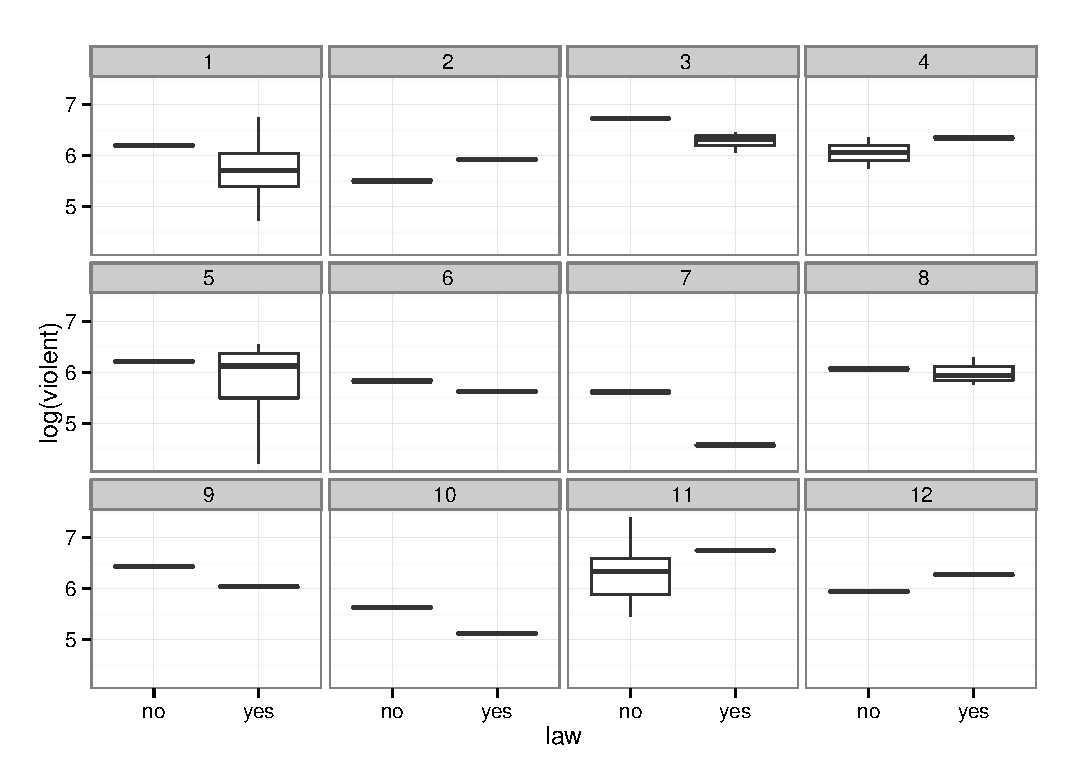
\includegraphics[width=\linewidth]{plots/unnamed-chunk-22} 

}



\end{knitrout}

Males do worse on average by 0.2693. Outlier slope detected in boxplot, but leaving it in. Looks like a significant gender effect.\\

Multilevel (very basic, each school has own inter./slope)\\
Level 1: $normexam_{ij} = a_{0i} + a_{1i} sex_{ij} + e_{ij}$\\
Level 2: $a_{0i} = b_{00} + e_{0i}$\\
          $a_{1i} = b_{10} + e_{1i}$\\
Combined: $normexam_{ij} = b_{00} + b_{10} sex_{ij} + [e_{ij}+e_{0i}+e_{1i}]$\\
\begin{knitrout}
\definecolor{shadecolor}{rgb}{0.969, 0.969, 0.969}\color{fgcolor}\begin{kframe}
\begin{alltt}
\hlfunctioncall{lmer}(normexam~sex+(sex|school), coed)
\end{alltt}
\begin{verbatim}
Linear mixed model fit by REML 
Formula: normexam ~ sex + (sex | school) 
   Data: coed 
  AIC  BIC logLik deviance REMLdev
 5836 5870  -2912     5816    5824
Random effects:
 Groups   Name        Variance Std.Dev. Corr   
 school   (Intercept) 0.18449  0.4295          
          sexM        0.00123  0.0351   -1.000 
 Residual             0.82187  0.9066          
Number of obs: 2169, groups: school, 35

Fixed effects:
            Estimate Std. Error t value
(Intercept)   0.0331     0.0789    0.42
sexM         -0.2614     0.0416   -6.28

Correlation of Fixed Effects:
     (Intr)
sexM -0.402
\end{verbatim}
\end{kframe}
\end{knitrout}

$b_{00}$ intercept (female score avg): .03311 (slightly above SFYS)\\
$b_{10}$ gender effect -.2614 (se=.04163) for males (similar to SFYS)\\
There is a significant gender gap in normexam.

\subsection*{part 2 d}
\emph{Note: I just saw the correction today (Thu) before class. There was no email about it and I finished the midterm before 2/12. I'm trying to correct the below, but I hope you are mindful that this is a quick fix.}

Here are some plots that help compare gender. The first one shows normexam for male and female and fits a line that goes through the means for each school. A horizontal line would indicate gender balance in normexam. (This also illustrates the problem with schools 47 and 43).\\
The second plot shows these individual lines and we see that these lines show a downwards trend, confirming that males have lower normexam scores.
\begin{knitrout}
\definecolor{shadecolor}{rgb}{0.969, 0.969, 0.969}\color{fgcolor}\begin{kframe}
\begin{alltt}
\hlfunctioncall{library}(lattice)
\hlfunctioncall{xyplot}(normexam ~ sex | school, type=\hlfunctioncall{c}(\hlstring{"p"}, \hlstring{"r"}), 
       index.cond=\hlfunctioncall{function}(x,y) 
           \{\hlfunctioncall{coef}(\hlfunctioncall{lm}(y ~ x))[1]\}, data=coed)
\end{alltt}
\end{kframe}

{\centering 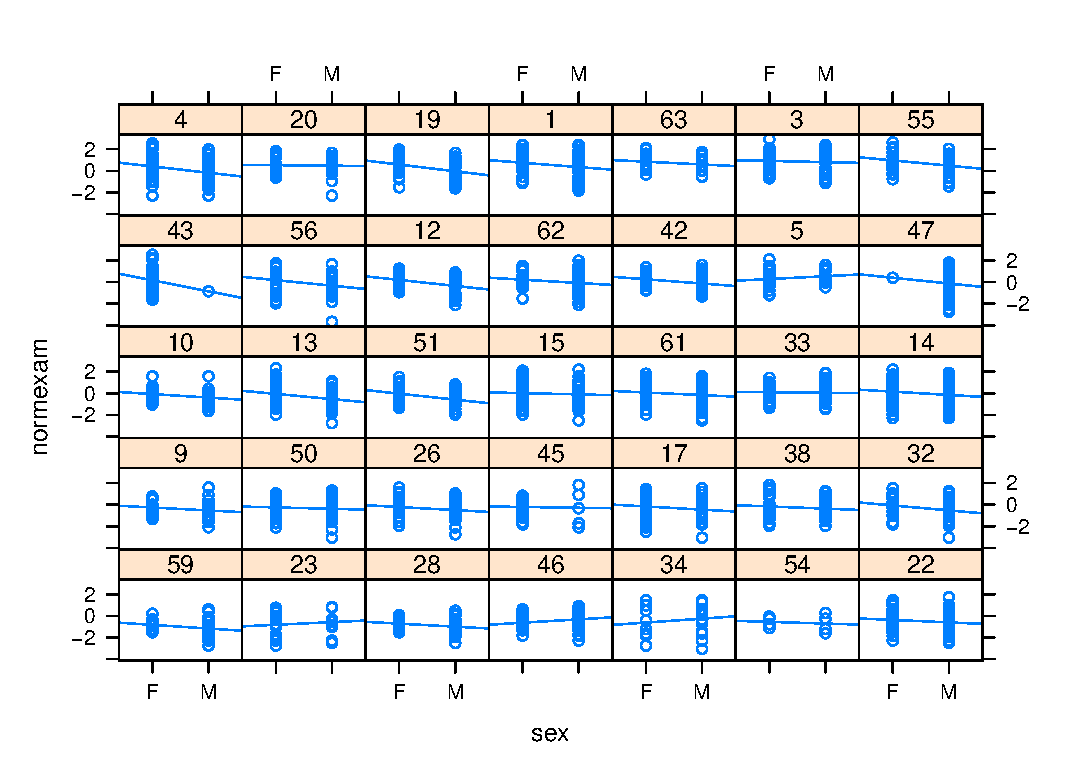
\includegraphics[width=\linewidth]{plots/unnamed-chunk-241} 

}


\begin{kframe}\begin{alltt}
\hlfunctioncall{xyplot}(normexam ~ sex , groups=school, type=\hlfunctioncall{c}(\hlstring{"r"}), 
       index.cond=\hlfunctioncall{function}(x,y) \{\hlfunctioncall{coef}(\hlfunctioncall{lm}(y ~ x))[1]\}, 
       data=coed, col = \hlfunctioncall{c}(\hlstring{"black"}))
\end{alltt}
\end{kframe}

{\centering 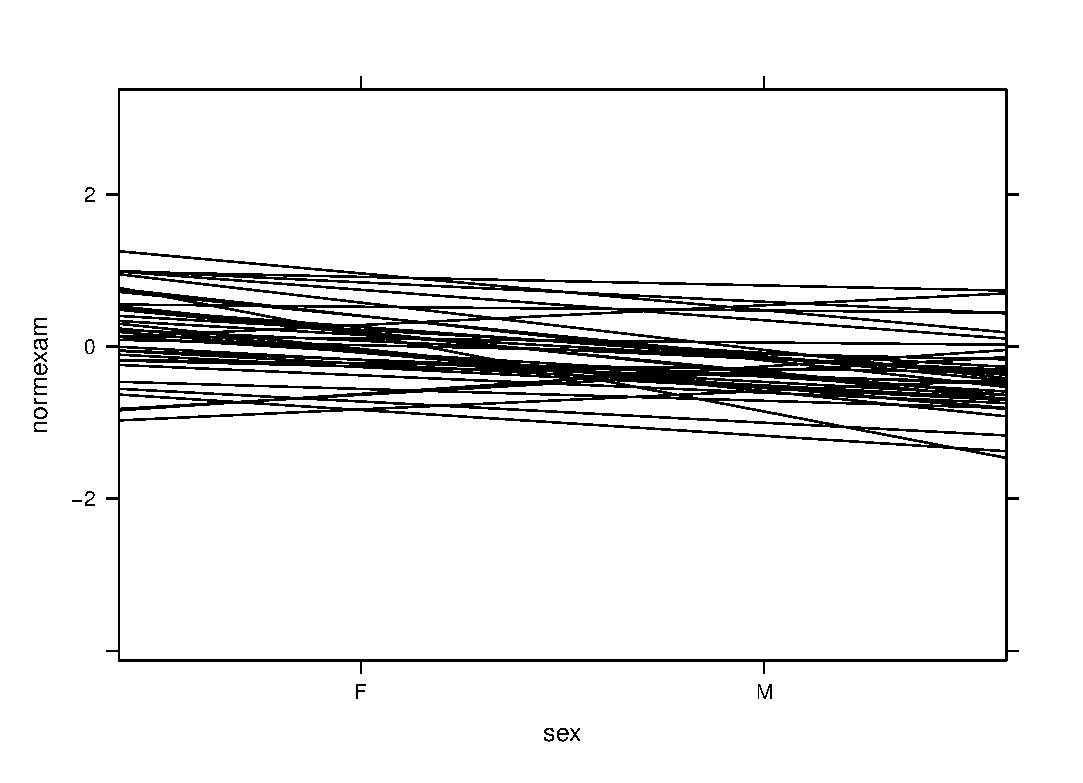
\includegraphics[width=\linewidth]{plots/unnamed-chunk-242} 

}



\end{knitrout}


Multilevel (intercept/slope depend on intake)\\
Level 1: $normexam_{ij} = a_{0i} + a_{1i} sex_{ij} + e_{ij}$\\
Level 2: $a_{0i} = b_{00} + b_{01} intake_i + e_{0i}$\\
          $a_{1i} = b_{10} + b_{11} intake_i + e_{1i}$\\
Combined: $normexam_{ij} = b_{00} + b_{01} intake_i + b_{10} sex_{ij} + b_{11} intake_i:sex_{ij} + [e_{ij}+e_{0i}+e_{1i}]$
\begin{knitrout}
\definecolor{shadecolor}{rgb}{0.969, 0.969, 0.969}\color{fgcolor}\begin{kframe}
\begin{alltt}
m1=\hlfunctioncall{lmer}(normexam~sex*schavg+(sex|school), coed)
\end{alltt}


{\ttfamily\noindent\color{warningcolor}{Warning: singular convergence (7)}}\begin{alltt}
m1
\end{alltt}
\begin{verbatim}
Linear mixed model fit by REML 
Formula: normexam ~ sex * schavg + (sex | school) 
   Data: coed 
  AIC  BIC logLik deviance REMLdev
 5822 5868  -2903     5794    5806
Random effects:
 Groups   Name        Variance Std.Dev. Corr   
 school   (Intercept) 0.09617  0.3101          
          sexM        0.00304  0.0551   -1.000 
 Residual             0.82298  0.9072          
Number of obs: 2169, groups: school, 35

Fixed effects:
            Estimate Std. Error t value
(Intercept)  0.05754    0.06088    0.95
sexM        -0.25863    0.04216   -6.13
schavg       0.90510    0.19566    4.63
sexM:schavg  0.00787    0.14071    0.06

Correlation of Fixed Effects:
            (Intr) sexM   schavg
sexM        -0.539              
schavg       0.054  0.002       
sexM:schavg  0.003  0.007 -0.552
\end{verbatim}
\end{kframe}
\end{knitrout}

$b_{00}$ intercept (intake=0,sex=F): -0.072\\
$b_{01}$ intake effect on intercept: est=0.909030, t=5 significant\\
$b_{10}$ gender effect/gap (for male): est=0.129313, t=6 significant\\
$b_{11}$ additional intake effect for males: not significant\\

Maybe better model without interaction effect fits better
\begin{knitrout}
\definecolor{shadecolor}{rgb}{0.969, 0.969, 0.969}\color{fgcolor}\begin{kframe}
\begin{alltt}
m2=\hlfunctioncall{lmer}(normexam~sex+schavg+(sex|school), coed)
\hlfunctioncall{anova}(m1,m2) \hlcomment{# simpler model favored by AIC and BIC}
\end{alltt}
\begin{verbatim}
Data: coed
Models:
m2: normexam ~ sex + schavg + (sex | school)
m1: normexam ~ sex * schavg + (sex | school)
   Df  AIC  BIC logLik Chisq Chi Df Pr(>Chisq)
m2  7 5808 5848  -2897                        
m1  8 5810 5855  -2897     0      1       0.97
\end{verbatim}
\end{kframe}
\end{knitrout}

Level 1: $normexam_{ij} \sim a_{0i} + a_{1i} sex_{ij} + e_{ij}$\\
Level 2: $a_{0i} = b_{00} + b_{01} intake_i + e_{0i}$\\
          $a_{1i} = b_{10} + e_{1i}$\\
Combined: $normexam_{ij} \sim b_{00} + b_{01} intake_i + b_{10} sex_{ij} + [e_{ij}+e_{0i}+e_{1i}]$
\begin{knitrout}
\definecolor{shadecolor}{rgb}{0.969, 0.969, 0.969}\color{fgcolor}\begin{kframe}
\begin{alltt}
m2
\end{alltt}
\begin{verbatim}
Linear mixed model fit by REML 
Formula: normexam ~ sex + schavg + (sex | school) 
   Data: coed 
  AIC  BIC logLik deviance REMLdev
 5818 5858  -2902     5794    5804
Random effects:
 Groups   Name        Variance Std.Dev. Corr   
 school   (Intercept) 0.09537  0.3088          
          sexM        0.00282  0.0531   -1.000 
 Residual             0.82262  0.9070          
Number of obs: 2169, groups: school, 35

Fixed effects:
            Estimate Std. Error t value
(Intercept)   0.0574     0.0607    0.95
sexM         -0.2585     0.0421   -6.14
schavg        0.9111     0.1632    5.58

Correlation of Fixed Effects:
       (Intr) sexM  
sexM   -0.534       
schavg  0.067  0.008
\end{verbatim}
\end{kframe}
\end{knitrout}

$b_{00}$ intercept (intake=0,sex=F): est=-0.07183\\
$b_{01}$ intake effect on intercept: est=0.91113, t=5.6 significant: higher intake associated with higher normalizd examscore\\
$b_{10}$ gender effect/gap (for male): est=0.12926, t=6.1 significant\\

The gender effect (and its significance in the model) is almost the same as before we added intake to the model. This suggests that the gender gap cannot be explained by the difference in intake, even though intake itself stands out as an important predictor in the model.

\end{document}
